\documentclass{article}

\usepackage[spanish]{babel}
\usepackage[utf8]{inputenc}
\usepackage{graphicx}
\usepackage{array}

\usepackage{yfonts}

\title{Mi documento}
\author{Víctor}

\usepackage{draftwatermark}
\SetWatermarkText{DRAFT}
\SetWatermarkScale{1}

\begin{document}

\maketitle{}
\newpage{}

\tableofcontents
\newpage{}

\section{Texto}

\yinipar{L}orem ipsum dolor sit amet, consectetur adipiscing elit. Sed sodales mauris eu accumsan volutpat. Curabitur cursus, erat et fringilla placerat, metus diam faucibus est, in malesuada ante sem nec turpis. Phasellus elementum leo eleifend velit commodo varius. Suspendisse elementum est sem, eget sagittis quam gravida vit\ae{}. Pr\ae{}sent dictum erat et risus dictum tincidunt. Nunc egestas euismod pulvinar. Quisque porttitor libero erat, eu scelerisque mauris ultricies at.

Pr\ae{}sent luctus ante in mollis scelerisque. Suspendisse euismod massa vel lectus viverra pulvinar. Donec id diam sit amet quam posuere malesuada. Aliquam eu neque sed nisi facilisis hendrerit. Fusce quis leo quis lorem vehicula imperdiet tincidunt sit amet justo. Suspendisse vel enim sem. Sed ac fringilla sapien. Vivamus vehicula sapien nulla, id ornare lorem placerat nec. Curabitur scelerisque eros in felis sagittis, sit amet blandit erat volutpat. Cum sociis natoque penatibus et magnis dis parturient montes, nascetur ridiculus mus. Quisque cursus ipsum in erat sollicitudin, ut porta neque scelerisque. Pr\ae{}sent auctor ex in maximus pulvinar. \AE{}nean sagittis turpis justo. Etiam pretium suscipit eleifend. \AE{}nean pellentesque vel turpis dignissim luctus. Morbi sit amet leo eu erat condimentum facilisis.

Pellentesque risus leo, convallis eu commodo eu, blandit sit amet tellus. Aliquam vehicula consequat sollicitudin. Nulla pellentesque eleifend sapien, a aliquet ante hendrerit a. Suspendisse leo urna, accumsan sit amet pellentesque sed, ultricies id augue. Vivamus imperdiet sollicitudin lacus non ultrices. M\ae{}cenas suscipit tempor nunc id consequat. Nulla interdum eget nulla condimentum dapibus. Duis nec efficitur arcu.

Proin sit amet accumsan augue. Nulla ac ipsum mauris. Pr\ae{}sent dignissim ante et dui sodales, sed semper est molestie. Duis porttitor condimentum diam. Vestibulum varius purus risus, non pharetra libero aliquet a. Interdum et malesuada fames ac ante ipsum primis in faucibus. Duis malesuada elementum molestie. Curabitur mollis nisl vel erat placerat placerat. Pellentesque dui ipsum, lobortis et eleifend nec, euismod nec enim. Nulla pulvinar gravida semper. Fusce a dapibus risus. Morbi ac est eget libero convallis rutrum.

Pr\ae{}sent viverra, ex sed rutrum tincidunt, tellus felis faucibus ex, egestas congue eros massa at metus. Aliquam vit\ae{} rhoncus sapien. Vivamus fringilla quis nibh id congue. In at felis ut nibh placerat cursus. Nam maximus eros quis sem feugiat, a aliquam purus tincidunt. Phasellus bibendum lobortis sapien, cursus elementum libero auctor sed. Class aptent taciti sociosqu ad litora torquent per conubia nostra, per inceptos himen\ae{}os. \AE{}nean faucibus sodales felis, non facilisis justo sodales eget. Nunc ornare pretium dolor, sit amet dignissim sapien vulputate in. In a eros sit amet tortor venenatis malesuada vit\ae{} vit\ae{} risus. Duis eu pharetra mauris. Nunc in ornare turpis, nec scelerisque felis. In et dolor quis dolor hendrerit dignissim non vel nibh. Donec ultricies porttitor augue, rhoncus faucibus tortor tempor sit amet. 

\section{Imagen}

Podemos ver una fotografia del Mont Blanc en la figura \ref{fig:montblanc}.

\begin{figure}
%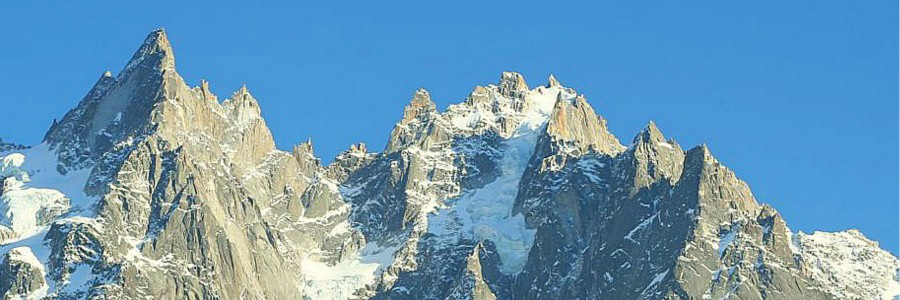
\includegraphics[width=\textwidth]{ejercicio1/montblanc}
\caption{Mont blanc.}
\label{fig:montblanc}
\end{figure}

\section{Tabla del tres}

\begin{table}
\center
\begin{tabular}{|r|l|}
\hline
3 x 1 & 3 \\ \hline
3 x 2 & 6 \\ \hline
3 x 3 & 9 \\ \hline
3 x 4 & 12 \\ \hline
3 x 5 & 15 \\ \hline
3 x 6 & 18 \\ \hline
3 x 7 & 21 \\ \hline
3 x 8 & 24 \\ \hline
3 x 9 & 27 \\ \hline
3 x 10 & 30 \\ \hline
\end{tabular}
\caption{Tabla del 3.}
\label{tab:tabla}
\end{table}

\end{document}